\documentclass{article}
\usepackage[utf8]{inputenc}
\usepackage{amsmath}
\usepackage{amsfonts}
\usepackage{tabularx}
\usepackage{layout}
\usepackage{geometry}
\usepackage{calc}
\usepackage{siunitx}
\usepackage{graphicx}
\usepackage{listings}
\usepackage{xcolor}
\usepackage{longtable}
\usepackage{soul}
\usepackage{physics}

\setlength{\hoffset}{0in}
\setlength{\voffset}{0in}
\setlength{\oddsidemargin}{0px}
\setlength{\headheight}{0em}
\setlength{\headsep}{0em}
\setlength{\marginparwidth}{0em}
\setlength{\marginparsep}{0em}
\setlength{\textheight}{\paperheight - 2in}
\setlength{\textwidth}{\paperwidth - 2in}
\setlength{\parskip}{1.5em}

\setlength{\parindent}{0px}
\setlength{\parskip}{2em}
\setlength{\tabcolsep}{0.2em}

\newcolumntype{C}{>{\centering\arraybackslash}X}


\newcommand{\hlc}[2][yellow]{{%
    \colorlet{foo}{#1}%
    \sethlcolor{foo}\hl{#2}}%
}

\newcommand{\question}[2]
{
    \begin{tabularx}{\linewidth}{lX}
        \textbf{#1)} & {#2}
    \end{tabularx} 
}

\newcommand{\silentquestion}[1]
{
    \begin{tabularx}{\linewidth}{lX}
        \phantom{\textbf{0)}} & {#1}
    \end{tabularx}
}

\newcommand{\expart}[1]
{
    \textbf{\underline{#1:}} \par 
}

% Pour les dt des intégrales
\newcommand*\dif{\mathop{}\!\mathrm{d}}

\begin{document}

\begin{tabularx}{\linewidth}{XCX}
    Chollet Arthur &\textbf{\underline{Compte rendu de la capacité numérique}}& 
\end{tabularx}

\expart{4.1: Circuit RC}
{
    Loi des mailles

    $iR+U_C=E \Longleftrightarrow  \dv{U_C}{t}+\frac{U_C}{RC}=E$

    Résulat (pas de 100):

    \begin{center}
      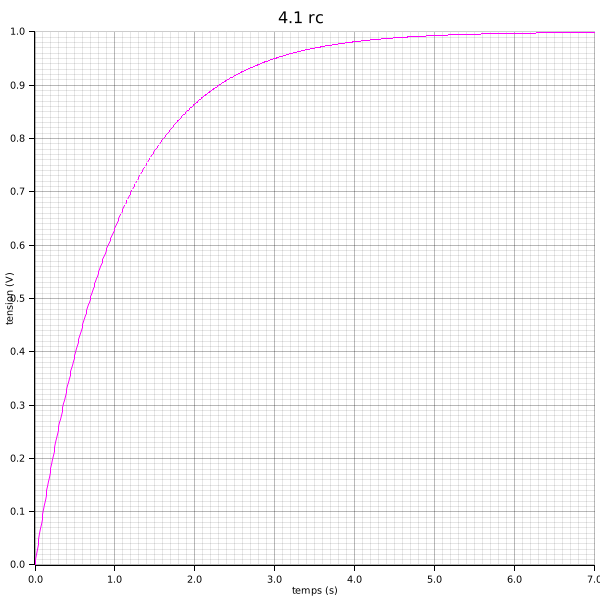
\includegraphics[height=35em]{images/rc}
    \end{center}
}

\pagebreak

\expart{4.1: Circuit RC}
{
    Schéma du circuit:

    \begin{center}
      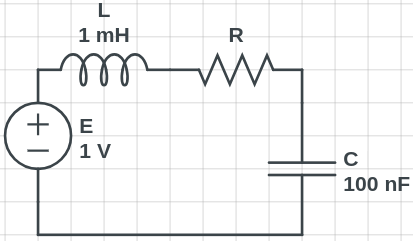
\includegraphics[height=15em]{images/rlc_schema.png}
    \end{center}

    \question{3}{
      Loi des mailles:

      $U_L+Ri+U_C=E$

      $L\dv{i}{t}+Ri+U_C=E$ or $i=C\dv{U_C}{t}$
      
      $\boxed{LC\dv[2]{U_C}{t}+RC\dv{U_C}{t}+U_C=E}$
    }

    \question{4}{
      $\dv[2]{U_C}{t}+\frac{R}{L}\dv{U_C}{t}+\frac{U_C}{LC}=\frac{E}{LC}$

      d'où: $\omega_0^2=\frac{1}{LC} \Longleftrightarrow \boxed{\omega_0=\frac{1}{\sqrt{LC}}}$

      et: $2Q\omega_0=\frac{R}{L} \Longleftrightarrow Q=\frac{R\sqrt{LC}}{2L} \Longleftrightarrow \boxed{Q=\frac{R}{2}\sqrt{\frac{C}{L}}}$
    }

    \question{5}{
      Équation caractétistique:
      $x^2+2Q\omega_0x+\omega_0^2=0$

      $\Delta=4Q^2\omega_0^2=4\omega_0^2=4\omega_0^2(Q^2-1)$

      \fbox{\begin{minipage}{1.0\textwidth}
          - \textbf{Apériodique} si: $\Delta>0 \Longleftrightarrow Q^2>1 \Longleftrightarrow Q>1 \Longleftrightarrow R>2\sqrt{\frac{L}{C}}$

          - \textbf{Critique} si: $\Delta=0 \Longleftrightarrow Q=1 \Longleftrightarrow R=2\sqrt{\frac{L}{C}}$

          - \textbf{Pseudo-périodique} si: $\Delta<0 \Longleftrightarrow Q<1 \Longleftrightarrow R<2\sqrt{\frac{L}{C}}$
      \end{minipage}}
    }

    \question{6}{
      Posons: $x_1=u$ et $x_2=\dot{u}$

      donc: $\dot{x_1}=\dot{u}=x_2$

      et: $\dot{x_2}=\ddot{u}=\omega_0^2E-2Q\omega_0\dot{u}-\omega_0^2u=\omega_0^2E-2Q\omega_0x_2-\omega_0^2x_1$

      Ainsi notre equation du second ordre est équivalent à ce système d'équations différentielle du 1er ordre:
      
      $\boxed{\begin{cases}
        \dot{x_1}=x_2 \\
        \dot{x_2}=\omega_0^2E-2Q\omega_0x_2-\omega_0^2x_1
      \end{cases}}$
    }
}


\end{document}
